\section{Computational determination of the channel capacity}
\label{supp_channcap}

In this section we detail the computation of the channel capacity of the simple
genetic circuit shown in \fref{fig5_channcap}. As detailed in
\secref{sec_channcap} the channel capacity is defined as the mutual information
between input $c$ and output $p$ maximized over all possible input distributions
$P(c)$ \cite{Shannon1948}. In principle there is an infinite number of input
distributions, so the task of finding $\hat{P}(c)$, the input distribution at
channel capacity, requires an algorithmic approach that guarantees the
convergence to this distribution. Tkačik, Callan and Bialek developed a clever
analytical approximation to find the $\hat{P}(c)$ distribution
\cite{Tkacik2008a}. The validity of their so-called small noise approximation
requires the standard deviation of the output distribution $P(p \mid c)$ to be
much smaller than the domain of the distribution. For our particular case such
condition is not satisfied given the spread of the inferred protein
distributions shown in \fref{fig4_maxent}.

Fortunately there exists a numerical algorithm to approximate $\hat{P}(c)$ for
discrete distributions. In 1972 Richard Blahut and Suguru Arimoto independently
came up with an algorithm mathematically shown to converge to $\hat{P}(c)$
\cite{Blahut1972}. To compute both, the theoretical and the experimental channel
capacity shown in \fref{fig5_channcap}, we implemented Blahut's algorithm. In
the following section we detail the definitions needed for the algorithm. Then
we detail how to compute the experimental channel capacity when the bins of the
distribution are not clear given the intrinsic arbitrary nature of microscopy
fluorescence measurements.

\subsection{Blahut's algorithm}

Following \cite{Blahut1972} we implemented the algorithm to compute the channel
capacity. We define $\bb{p_c}$ to be an array containing the probability of each
of the input inducer concentrations (twelve concentrations, See \mrm{Methods}).
Each entry $j$ of the array is then of the form
\begin{equation}
  p_c^{(j)} = P(c = c_j),
\end{equation}
with $j \in \{1, 2, \ldots, 12 \}$. The objective of the algorithm is to find
the entries $p_c^{(j)}$ that maximize the mutual information between inputs and
outputs. We also define $\bb{Q}$ to be a $\vert \bb{p_c} \vert$ by
$\vert \bb{p_{p \mid c}} \vert$ matrix, where $\vert \cdot \vert$ specifies the
length of the array, and $\bb{p_{p \mid c}}$ is an array containing the
probability distribution of an output given a specific value of the input. In
other words, the matrix $\bb{Q}$ recollects all of the individual output
distribution arrays $\bb{p_{p \mid c}}$ into a single object. Then each entry
of the matrix $\bb{Q}$ is of the form
\begin{equation}
  Q^{(i, j)} = P(p = p_i \mid c = c_j).
\end{equation}

For the case of the theoretical predictions of the channel capacity (Solid
lines in \fref{fig5_channcap}) the entries of matrix $\bb{Q}$ are given by the
inferred maximum entropy distributions as shown in \fref{fig4_maxent}. In the
next section we will discuss how to define this matrix for the case of the
single-cell fluorescence measurements. Having defined these matrices we proceed
to implement the algorithm shown in Figure 1 of \cite{Blahut1972}.

\subsection{Channel capacity from arbitrary units of fluorescence}

A difficulty when computing the channel capacity between inputs and outputs from
experimental data is that ideally we would like to compute
\begin{equation}
C(g; c) \equiv \max_{P(c)} I(g; c),
\end{equation}
where $g$ is the gene expression level, and $c$ is the inducer concentration.
But in reality we are computing
\begin{equation}
C(f(g); c) \equiv \max_{P(c)} I(f(g); c),
\end{equation}
where $f(g)$ is a function of gene expression that has to do with our mapping
from the YFP copy number to some arbitrary fluorescent value as computed from
the images taken with the microscope.

The data processing inequality, as derived by Shannon himself, tells us that
for a Markov chain of the form $c \rightarrow g \rightarrow f(g)$ it must be
true that \cite{Shannon1948}
\begin{equation}
I(g; c) \geq I(f(g); c),
\end{equation}
meaning that we can at best not lose information when mapping from the real
relationship between gene expression and inducer concentration to a fluorescence
value.

On top of that, given the limited number of samples that we have access to when
computing the channel capacity, there is a bias in our estimate given this
undersampling. The definition of accurate unbiased descriptors of the mutual
information is still an area of active research. For our purposes we will use
the method described in \cite{Cheong2011a}.

The basic idea of the method is to write the mutual information as a series
expansion in terms of inverse powers of the sample size, i.e.
\begin{equation}
I_{\text{biased}} = I_\infty + \frac{a_1}{N} + \frac{a_2}{N^2} + \cdots,
\end{equation}
where $I_{\text{biased}}$ is the biased estimate of the mutual information as
computed from experimental data, $I_\infty$ is the quantity we would like to
estimate, being the unbiased mutual information when having access to infinity
number of experimental samples, and the coefficients $a_i$ depend on the
underlying distribution of the signal and the response.

In principle for a good number of data points the terms of higher order become
negligible. So we can write the mutual information as
\begin{equation}
I_{\text{biased}} \approx I_\infty + \frac{a_1}{N} + \mathcal{O}(N^{-2}).
\label{seq_mutual_biased}
\end{equation}
This means that when computing the mutual information for varying number of
samples, by taking subsamples of the experimental data, we expect to find a
linear relationship as a function of the inverse of these number of data points.
From this linear relationship the intercept is a bias-corrected estimate of the
mutual information. We can therefore bootstrap the data by taking different
sample sizes and then use the Blahut-Arimoto algorithm we implemented earlier to
estimate the biased channel capacity. We can then fit a line and extrapolate for
when $1/N = 0$ which corresponds to our unbiased estimate of the channel
capacity.

Let's go through each of the steps to illustrate the method.
\fref{sfig_fluor_dist} show a typical data set for a strain with an O2 binding
site ($\eR = -13.9 \; k_BT$) and $R = 260$ repressors per cell. Each of the
distributions in arbitrary units is binned into a specified number of bins to
build matrix $\bb{Q}$.

\begin{figure}[h!]
	\centering \includegraphics
  {../fig/channel_capacity_experiment/O2_RBS1027_distribution_microscopy.pdf}
	\caption{\textbf{Single cell fluorescence distributions for different inducer
	concentrations.} Fluorescence distribution histogram (A) and cumulative
	distribution function (B) for a strain with 260 repressors per cell and a
	binding site with binding energy $\eR = -13.9\; k_BT$. The different curves
	show the single cell fluorescence distributions under the 12 different IPTG
	concentrations used throughout this work. The triangles in (A) show the mean
	of each of the distributions.}
  \label{sfig_fluor_dist}
\end{figure}

Given a specific number of bins used to construct $\bb{Q}$, we subsample a
fraction of the data and compute the channel capacity for such matrix using the
Blahut-Arimoto algorithm. \fref{sfig_channcap_bootstrap} shows an example where
50\% of the data on each distribution from \fref{sfig_fluor_dist} was sampled
and binned into 100 equal bins. The counts on each of these bins are then
normalized and used to build matrix $\bb{Q}$ that is then fed to the
Blahut-Arimoto algorithm. We can see that for these 200 bootstrap samples the
channel capacity varies by $\approx$ 0.1 bits. Not a significant variability,
nevertheless is important to bootstrap the data multiple times to get a better
estimate of the channel capacity.

\begin{figure}[h!]
	\centering \includegraphics
  {../fig/channel_capacity_experiment/bootstrap_ecdf_channcap.pdf}
  \caption{\textbf{Channel capacity bootstrap for experimental data.} Cumulative
  distribution function of the resulting channel capacity estimates obtained by
  subsampling 200 times 50\% of each distribution shown in
  \fref{sfig_fluor_dist}, binning it into 100 bins, and feeding the resulting
  $\bb{Q}$ matrix to  the Blahut-Arimoto algorithm.}
  \label{sfig_channcap_bootstrap}
\end{figure}

\eref{seq_mutual_biased} tells us that if we subsample each of the distributions
from \fref{sfig_fluor_dist} at different fractions, and plot them as a function
of the inverse sample size we will find a linear relationship if the expansion
of the mutual information is valid. To test this idea we repeated the bootstrap
estimate of \fref{sfig_channcap_bootstrap} sampling 10\%, 20\%, and so on until
taking 100\% of the data. We repeated this for different number of bins since a
priori for arbitrary units of fluorescence we do not have a way to select the
optimal number of bins. \fref{sfig_channcap_lin_reg} shows the result of these
estimates. We can see that the linear relationship proposed in
\eref{seq_mutual_biased} holds true for all number of bins selected. We also
note that the value of the intercept of the linear regression varies depending
on the number of bins.

\begin{figure}[h!]
	\centering \includegraphics
  {../fig/channel_capacity_experiment/I_infty_lin_reg.pdf}
  \caption{\textbf{Inverse sample size vs channel capacity.} As indicated in
  \eref{seq_mutual_biased} if the channel capacity obtained for different
  subsample sizes of the data is plotted against the inverse sample size there
  must exist a linear relationship between these variables. Here we perform 15
  bootstrap samples of the data from \fref{sfig_fluor_dist}, bin these samples
  using  different number of bins, and perform a linear regression (solid lines)
  between the bootstrap channel capacity estimates, and the inverse sample
  size.}
  \label{sfig_channcap_lin_reg}
\end{figure}

To address the variability in the estimates of the unbiased channel capacity
$I_\infty$ we again follow the methodology suggested in \cite{Cheong2011a}. We
perform the data subsampling and computation of the channel capacity for a
varying number of bins. As a control we perform the same procedure with shuffled
data, where the structure that connects the fluorescence distribution to the
inducer concentration input is lost. The expectation is that this control should
give a channel capacity of zero if the data is not ``over-binned.'' Once the
number of bins is too high, we would expect some structure to emerge in the data
that would cause the Blahut-Arimoto algorithm to return non-zero channel
capacity estimates.

\fref{sfig_bins_channcap} shows the result of the unbiased channel capacity
estimates obtained for the data shown in \fref{sfig_fluor_dist}. For the blue
curve we can distinguish three phases:
\begin{enumerate}
  \item A rapid increment from 0 bits to about 1.5 bits as the number of bins
  increases.
  \item A flat region between $\approx$ 50 and 1000 bins.
  \item A second rapid increment for large number of bins.
\end{enumerate}
We can see that the randomized data presents two phases only:
\begin{enumerate}
  \item A flat region where there is, as expected no information being processed
  since the structure of the data was lost when the data was shuffled.
  \item A region with fast growth of the channel capacity as the over-binning
  generates separated peaks on the distribution, making it look like there is
  structure in the data.
\end{enumerate}
We take the flat region of the experimental data ($\approx$ 100 bins) to be our
best unbiased estimate of the channel capacity from this experimental dataset.

\begin{figure}[h!]
	\centering 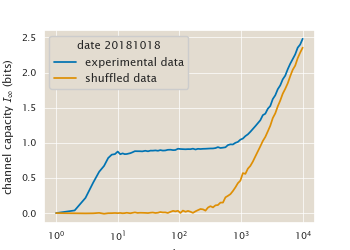
\includegraphics
  {../fig/channel_capacity_experiment/bins_vs_channcap.pdf}
  \caption{\textbf{Channel capacity as a function of the number of bins.}
  Unbiased channel capacity estimates obtained from linear regressions as in
  \fref{sfig_channcap_lin_reg}. The blue curve show the estimates obtained from
  the data shown in \fref{sfig_fluor_dist}. The orange curve is generated from
  estimates where the same data is shuffled, loosing the relationship between
  fluroescence distributions and inducer concentration.}
  \label{sfig_bins_channcap}
\end{figure}
